\PassOptionsToPackage{unicode=true}{hyperref} % options for packages loaded elsewhere
\PassOptionsToPackage{hyphens}{url}
%
\documentclass[]{article}
\usepackage{lmodern}
\usepackage{amssymb,amsmath}
\usepackage{ifxetex,ifluatex}
\usepackage{fixltx2e} % provides \textsubscript
\ifnum 0\ifxetex 1\fi\ifluatex 1\fi=0 % if pdftex
  \usepackage[T1]{fontenc}
  \usepackage[utf8]{inputenc}
  \usepackage{textcomp} % provides euro and other symbols
\else % if luatex or xelatex
  \usepackage{unicode-math}
  \defaultfontfeatures{Ligatures=TeX,Scale=MatchLowercase}
\fi
% use upquote if available, for straight quotes in verbatim environments
\IfFileExists{upquote.sty}{\usepackage{upquote}}{}
% use microtype if available
\IfFileExists{microtype.sty}{%
\usepackage[]{microtype}
\UseMicrotypeSet[protrusion]{basicmath} % disable protrusion for tt fonts
}{}
\IfFileExists{parskip.sty}{%
\usepackage{parskip}
}{% else
\setlength{\parindent}{0pt}
\setlength{\parskip}{6pt plus 2pt minus 1pt}
}
\usepackage{hyperref}
\hypersetup{
            pdfborder={0 0 0},
            breaklinks=true}
\urlstyle{same}  % don't use monospace font for urls
\usepackage[margin=1in]{geometry}
\usepackage{graphicx,grffile}
\makeatletter
\def\maxwidth{\ifdim\Gin@nat@width>\linewidth\linewidth\else\Gin@nat@width\fi}
\def\maxheight{\ifdim\Gin@nat@height>\textheight\textheight\else\Gin@nat@height\fi}
\makeatother
% Scale images if necessary, so that they will not overflow the page
% margins by default, and it is still possible to overwrite the defaults
% using explicit options in \includegraphics[width, height, ...]{}
\setkeys{Gin}{width=\maxwidth,height=\maxheight,keepaspectratio}
\setlength{\emergencystretch}{3em}  % prevent overfull lines
\providecommand{\tightlist}{%
  \setlength{\itemsep}{0pt}\setlength{\parskip}{0pt}}
\setcounter{secnumdepth}{0}
% Redefines (sub)paragraphs to behave more like sections
\ifx\paragraph\undefined\else
\let\oldparagraph\paragraph
\renewcommand{\paragraph}[1]{\oldparagraph{#1}\mbox{}}
\fi
\ifx\subparagraph\undefined\else
\let\oldsubparagraph\subparagraph
\renewcommand{\subparagraph}[1]{\oldsubparagraph{#1}\mbox{}}
\fi

% set default figure placement to htbp
\makeatletter
\def\fps@figure{htbp}
\makeatother

\usepackage{ctex}
\usepackage{xcolor}
\usepackage{fancyhdr}
\pagestyle{fancy}
\cfoot{\thepage}
\usepackage{sectsty}
\definecolor{glaucous}{rgb}{0.38, 0.51, 0.71}
\definecolor{lavenderblush}{rgb}{1.0, 0.94, 0.96}
\usepackage{enumitem}% http://ctan.org/pkg/enumitem
\usepackage[empty]{fullpage}% http://ctan.org/pkg/fullpage
\usepackage{color}% http://ctan.org/pkg/color
\usepackage{hyperref}% http://ctan.org/pkg/hyperref
\usepackage{geometry}
\geometry{a4paper,left=1.5cm,right=1.5cm,top=0.3cm,bottom=0.3cm}
\usepackage{blindtext}
\usepackage[center]{caption}
\usepackage{subfigure}
\usepackage{float}
\usepackage{graphicx}
\usepackage{booktabs}
\usepackage[justification=centering]{caption}
\usepackage{threeparttable}
\usepackage{longtable}
\usepackage{array}
\usepackage{multirow}
\usepackage{wrapfig}
\usepackage{float}
\usepackage{colortbl}
\usepackage{pdflscape}
\usepackage{tabu}
\usepackage{threeparttable}
\usepackage{threeparttablex}
\usepackage[normalem]{ulem}
\usepackage{makecell}
\usepackage{xcolor}
\linespread{1.5}
\setlength{\parskip}{0.5em}
\setlength{\footskip}{20pt}
\usepackage{booktabs}
\usepackage{longtable}
\usepackage{array}
\usepackage{multirow}
\usepackage{wrapfig}
\usepackage{float}
\usepackage{colortbl}
\usepackage{pdflscape}
\usepackage{tabu}
\usepackage{threeparttable}
\usepackage{threeparttablex}
\usepackage[normalem]{ulem}
\usepackage{makecell}
\usepackage{xcolor}

\author{}
\date{\vspace{-2.5em}}

\begin{document}

\captionsetup[figure]{name={图},labelsep=space} 
\captionsetup[table]{name={表},labelsep=space} 
\fontsize{14}{14}
\selectfont
\vspace{-10truemm}

\newcommand{\resheading}[1]{%
  \noindent\fcolorbox{lavenderblush}{lavenderblush}{\makebox[\dimexpr\textwidth-2\fboxsep-2\fboxrule][l]{\textbf{~#1}}}%
}

\begin{center}

\includegraphics[height=2cm]{./input/logo2.png} 
\end{center}

\vspace{-5truemm}

\begin{center}
\fontsize{40}{40}
\textcolor{glaucous}{\textbf{新冠早报}}
\end{center}

\begin{center}
\fontsize{20}{20}
{\textcolor{glaucous}{\textbf{第13期 \space 4月8日}}}
\end{center}

%
  \noindent\fcolorbox{lavenderblush}{lavenderblush}{\makebox[\dimexpr\textwidth-2\fboxsep-2\fboxrule][l]{\textbf{~\Large 每日新闻}}}%

\vspace{-5mm}

\hypertarget{section}{%
\subsection{\texorpdfstring{\textcolor{glaucous}{\Large 国际}}{}}\label{section}}

\vspace{-3mm}

\textbf{\textcolor{glaucous}{英国广播公司(BBC)}}:
\textbf{纽约州长制定五月重新开放的计划 }

据当地时间4月28日报道,美国纽约州州长安德鲁·库莫称,纽约州部分地区若满足解禁条件(包括连续14天新冠病例下降),则5月15日可以开始放宽新冠限制措施。但医院容纳量在70%以上,或新冠传染率高于1.1的地区都不能重新开放。如果制造业和建筑业能够采取充分预防措施,它们将会是首批重新开放的企业。

\textbf{\textcolor{glaucous}{美国有线电视新闻网(CNN)}} :
\textbf{特朗普命令肉类加工厂保持开放}

当地时间4月28日,美国总统特朗普称,他将根据《国防生产法》签署一项五页的行政命令,保持肉类加工厂在冠状病毒大流行中继续开放。此命令是在一些公司(例如泰森食品公司)考虑只开放其20%的设施之后签署的。美国政府还将与劳工部合作,发布对有关对肉类加工厂雇员的居家指导。

\textbf{\textcolor{glaucous}{英国广播公司(BBC)}} :
\textbf{英国将扩大面向护理机构员工和65岁以上老人的新冠测试}

当地时间4月28日,英国卫生部长马特·汉考克称,英国所有疗养院居民和工作人员,不论是否有症状,都将符合新冠检测的资格。从4月29日开始,所有有症状的65岁以上以及必须出门上班的人,也可以接受检查。汉考克称,现在英国每日测试能力高达73,400,到五月,政府每天将进行10万次测试。

\textbf{\textcolor{glaucous}{纽约时报(New York Times)}} :
\textbf{西班牙,法国和希腊公布放宽新冠限制措施计划 }

据美东时间4月28日报道,西班牙总理佩德罗·桑切斯宣布,自5月2日起,成年人可以在户外运动。限制措施的放宽将因地区而异,但学校不会在9月之前重新开放。希腊总理基里亚科斯·米佐塔基斯表示,5月4日开始,希腊人可以自由离开家,届时一些商店将重新营业,但沙龙将仅通过预约开放,教堂将开放但不能举行礼拜,人们可以去海滩运动,高中生将从5月11日起分阶段重返学校。法国总理爱德华·菲利普称,如果新冠疫情持续得到控制,政府将在5月11日开始放宽限制措施,并于6月2日重新评估这些措施。

\textbf{\textcolor{glaucous}{英国广播公司(BBC)}} :
\textbf{特朗普承诺向尼日利亚提供呼吸机 }

当地时间4月28日,尼日利亚政府官员在每日新闻发布会上表示,既美国总统特朗普承诺向厄瓜多尔提供呼吸机后,其首次承诺向尼日利亚等西非国家提供呼吸机,帮助其应对冠状病毒的流行。

\textbf{\textcolor{glaucous}{NA}} : \textbf{NA}

NA

\vspace{-5mm}

\hypertarget{section-1}{%
\subsection{\texorpdfstring{\textcolor{glaucous}{\Large 国内}}{}}\label{section-1}}

\vspace{-3mm}

\textbf{\textcolor{glaucous}{中国新闻网}}:
\textbf{小汤山医院新冠肺炎患者全部``清零'' }

北京时间4月28日上午,随着最后两名患者顺利出院,小汤山医院新冠肺炎患者全部``清零'',首批912名医务人员零感染回家。

\textbf{\textcolor{glaucous}{美国公共广播电台(NPR)}}:
\textbf{北京批评印度取消中国抗体检测试剂盒订单是``不公正''的决定}

当地时间4月27日,印度医药研究议会建议停止使用从中国广州万孚生物技术和珠海丽珠试剂公司生产的抗体检测试剂盒,并将65万个抗体检测试剂盒的订单退回中国供应商。该议会声称这批抗体检测试剂盒的检测敏感性差异较大。北京时间4月28日,中国驻新德里使馆发言人吉荣批评印度取消进口中国抗体检测试剂盒订单的决定,坚持测试剂盒已经过验证和批准。他在声明中称:``某些人将中国产品标记为`有缺陷',并以固有偏见看待这些问题是不公平和不负责任的。''

\vspace{5mm}
%
  \noindent\fcolorbox{lavenderblush}{lavenderblush}{\makebox[\dimexpr\textwidth-2\fboxsep-2\fboxrule][l]{\textbf{~\Large 疫情观察}}}%

\begin{small}
{数据源:约翰霍普金斯大学,The COVID Tracking Project \quad   数据截止至:北京时间3月28日 早4:00}
\end{small}

\vspace{-7mm}

\hypertarget{section-2}{%
\section{\texorpdfstring{\textcolor{glaucous}{一、世界疫情}}{}}\label{section-2}}

\vspace{-5mm}

\(\quad\)截至北京时间4月29日早7:00,全球累计确诊病例已经达到3,111,730例,累计死亡216,857例。25个国家累计确诊病例超过15,000例。总体来看,欧洲与北美仍是累计确诊病例数最多的地区。英国的累计确诊数突破十六万,超过德国进入世界前五位。爱尔兰的累计确诊病例接近两万(19,877),粗发病率达403/10万人,已经超过意大利与瑞士,疫情正在迅速恶化。俄罗斯的累计确诊病例数超过伊朗,跃升至世界第八位。
中东地区除伊朗外,沙特阿拉伯累计确诊病例超过两万,以色列,巴基斯坦,卡塔尔与阿联酋的累计确诊均已超过一万例。东欧地区白俄罗斯病例增长迅速(累计确诊12,208例),较上周(4月22日)接近翻倍,粗发病率到达129/10万,超过湖北。中东及东欧各国变化表明,疫情在欧亚大陆自西向东多点扩散。(表1)

\begin{figure}[H]
\caption{世界疫情分布图} %最终文档中希望显示的图片标题
\centering
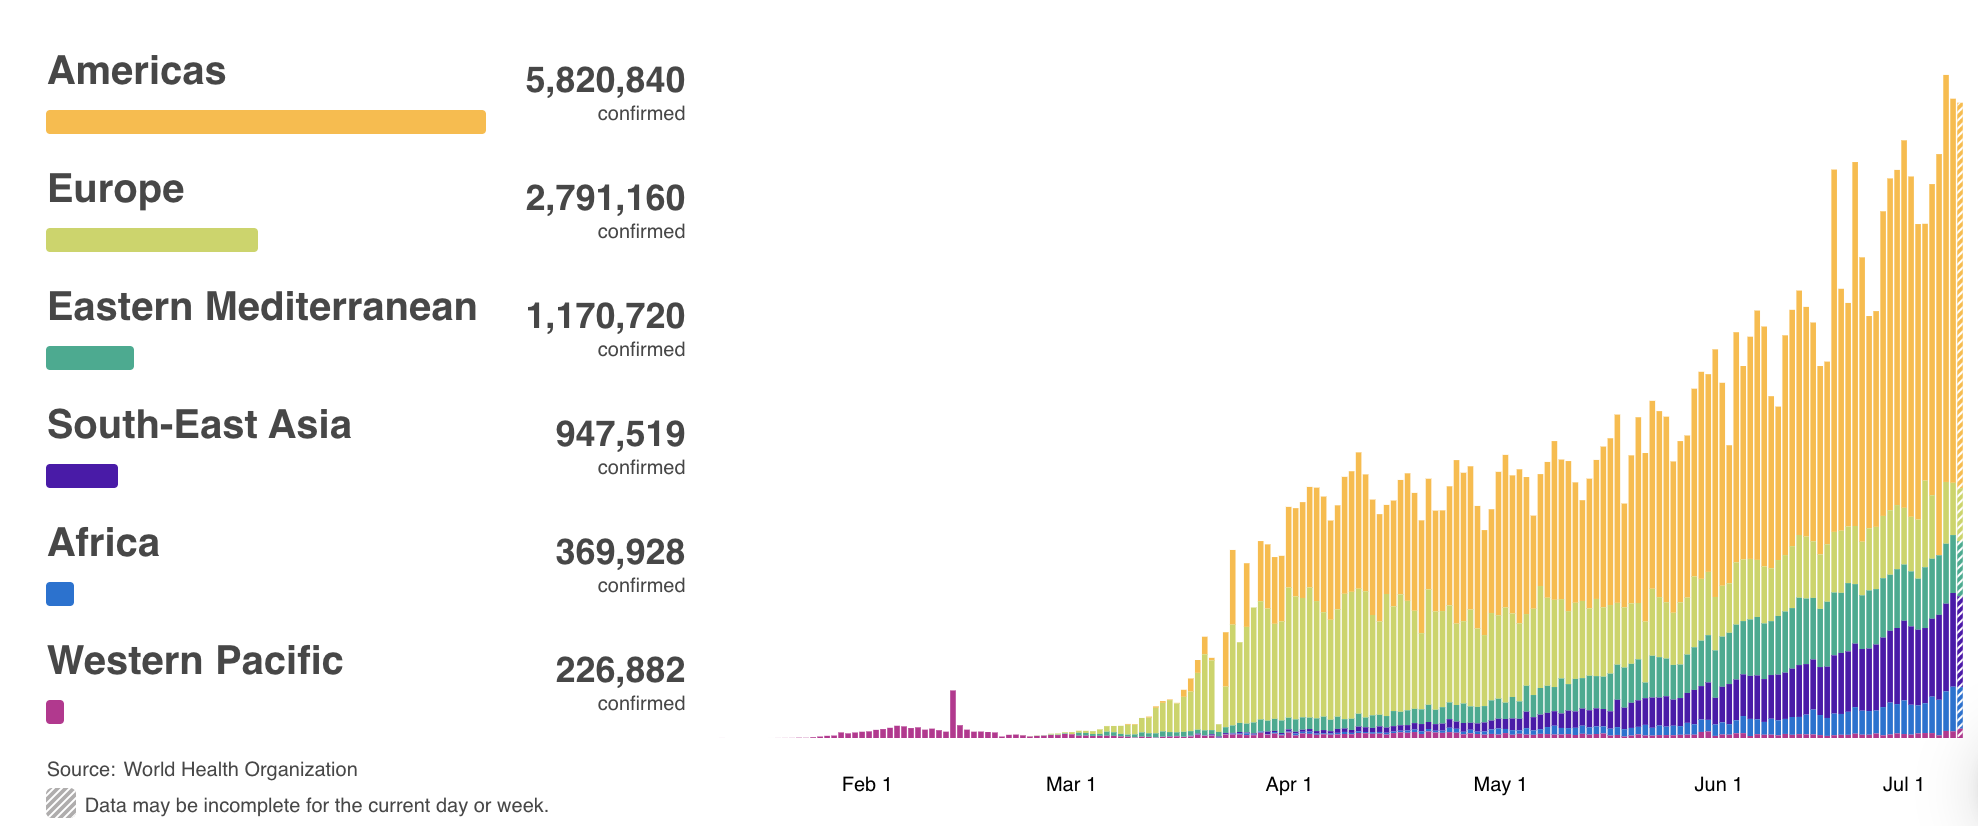
\includegraphics[]{./input/covid1.png} %插入图片,[]中设置图片大小,{}中是图片文件名
\label{} %用于文内引用的标签
\end{figure}

\begin{table}[H]
    
    \begin{minipage}{.4\linewidth}
    \centering
    \captionsetup{justification=centering}
    \caption{累计确诊前十位国家}
      \vspace{-0.5\baselineskip}
      \centering
      \captionsetup{justification=centering} \begin{table}[H]
\centering
\begin{tabular}{rlrr}
\toprule
  & 国家(地区) & 累计确诊病例 & 粗发病率*\\
\midrule
\rowcolor{gray!6}  1 & 美国 US & 2,291,353 & 692\\
2 & 巴西 Brazil & 1,083,341 & 510\\
\rowcolor{gray!6}  3 & 俄罗斯 Russia & 591,465 & 405\\
4 & 印度 India & 425,282 & 31\\
\rowcolor{gray!6}  5 & 英国 UK & 306,761 & 452\\
6 & 秘鲁 Peru & 251,338 & 762\\
\rowcolor{gray!6}  7 & 智利 Chile & 246,963 & 1,292\\
8 & 西班牙 Spain & 246,504 & 527\\
\rowcolor{gray!6}  9 & 意大利 Italy & 238,720 & 395\\
10 & 伊朗 Iran & 207,525 & 247\\
\bottomrule
\end{tabular}
\end{table} \end{minipage}
    \begin{minipage}{.7\linewidth}
    \centering
    \captionsetup{justification=centering}
     \caption{粗发病率前十位国家}
     \vspace{-0.5\baselineskip}
      \centering
    \captionsetup{justification=centering} \begin{table}[H]
\centering
\begin{tabular}{rlrr}
\toprule
  & 国家(地区) & 粗发病率* & 累计确诊病例\\
\midrule
\rowcolor{gray!6}  1 & 卡塔尔 Qatar & 3,068 & 88,403\\
2 & 圣马力诺** San Marino & 2,054 & 697\\
\rowcolor{gray!6}  3 & 梵蒂冈** Holy See & 1,498 & 12\\
4 & 智利 Chile & 1,292 & 246,963\\
\rowcolor{gray!6}  5 & 巴林 Bahrain & 1,279 & 21,764\\
6 & 安道尔** Andorra & 1,107 & 855\\
\rowcolor{gray!6}  7 & 科威特 Kuwait & 943 & 40,291\\
8 & 秘鲁 Peru & 762 & 251,338\\
\rowcolor{gray!6}  9 & 新加坡 Singapore & 723 & 42,313\\
10 & 亚美尼亚 Armenia & 695 & 20,588\\
\bottomrule
\end{tabular}
\end{table} \end{minipage}
    
    \begin{tablenotes}
        \fontsize{12}{12}
        \selectfont
        \item 注:粗发病率定义:在一定时间内,特定范围人群中某病新发生的病例出现的频率。计算方式:(累计确诊病例/人口)×10万;**国家人口不足10万人,圣马力诺33,931人,梵蒂冈801人,安道尔77,265人。  %此处加入注释信息
      \end{tablenotes}
\end{table}

\newpage

\(\quad\)从日新增病例数来看,美国与俄罗斯仍就占据世界前二,值得注意的是,俄罗斯的日新增病例呈明显上升趋势,该国疫情发展不容乐观。巴西日新增突破4000例,首次进入世界前三;秘鲁日新增接近2500例,两国日新增较上周均接近翻倍(4月22日:巴西2678例,秘鲁1413例),显示疫情在南美洲呈爆发性增长趋势。
白俄罗斯的单日新增919例,疫情在该国发展需要进一步关注。另一方面,西班牙与意大利的日新增病例持续下降,表明疫情逐步得到较好控制。(表2和图2)

\(\quad\)从死亡病例数来看,美国仍是累计死亡病例最多的国家,虽日新增死亡呈现波动下降趋势。巴西累计死亡病例突破5000例,超过中国,日新增死亡也呈逐日上升态势。此外,意大利、西班牙、法国、德国等欧洲国家日新增死亡病例数呈现下降趋势,提示疫情在欧洲逐步缓解。
(表3和图3)

\begin{table}[H]
    \begin{minipage}{.4\linewidth}
    \centering
    \captionsetup{justification=centering}
    \caption{日新增病例前十位国家}
    \vspace{-0.5\baselineskip}
      \centering
    \captionsetup{justification=centering} \begin{table}[H]
\centering
\begin{tabular}{rlr}
\toprule
  & 国家 & 当日新增病例\\
\midrule
\rowcolor{gray!6}  1 & 美国 US & 11,474\\
2 & 俄罗斯 Russia & 7,586\\
\rowcolor{gray!6}  3 & 智利 Chile & 4,608\\
4 & 孟加拉国 Bangladesh & 3,480\\
\rowcolor{gray!6}  5 & 沙特 Saudi Arabia & 3,393\\
6 & 瑞典 Sweden & 2,889\\
\rowcolor{gray!6}  7 & 伊朗 Iran & 2,573\\
8 & 伊拉克 Iraq & 1,808\\
\rowcolor{gray!6}  9 & 阿曼 Oman & 1,605\\
10 & 土耳其 Turkey & 1,212\\
\bottomrule
\end{tabular}
\end{table} \end{minipage}
    \begin{minipage}{.6\linewidth}
    \centering
    \captionsetup{justification=centering}
     \caption{累计死亡病例前十位国家}
     \vspace{-0.5\baselineskip}
      \centering
    \captionsetup{justification=centering} \begin{table}[H]
\centering
\begin{tabular}{rlrrr}
\toprule
  & 国家 & 累计死亡病例 & 较昨日新增 & 病死率\%\\
\midrule
\rowcolor{gray!6}  1 & 美国 US & 120,106 & 137 & 5.2\\
2 & 巴西 Brazil & 50,591 & 0 & 4.7\\
\rowcolor{gray!6}  3 & 英国 UK & 42,731 & 14 & 13.9\\
4 & 意大利 Italy & 34,657 & 23 & 14.5\\
\rowcolor{gray!6}  5 & 法国 France & 29,643 & 0 & 15.0\\
6 & 西班牙 Spain & 28,752 & 0 & 11.7\\
\rowcolor{gray!6}  7 & 墨西哥 Mexico & 21,825 & 0 & 12.1\\
8 & 印度 India & 13,699 & 0 & 3.2\\
\rowcolor{gray!6}  9 & 伊朗 Iran & 9,742 & 119 & 4.7\\
10 & 比利时 Belgium & 9,696 & 0 & 16.0\\
\bottomrule
\end{tabular}
\end{table} \end{minipage} 
\end{table}

\begin{figure}[H]
\centering
\begin{minipage}[b]{0.45\linewidth}
\caption{日新增确诊病例国家趋势图\\(中国及其他前五位国家)}
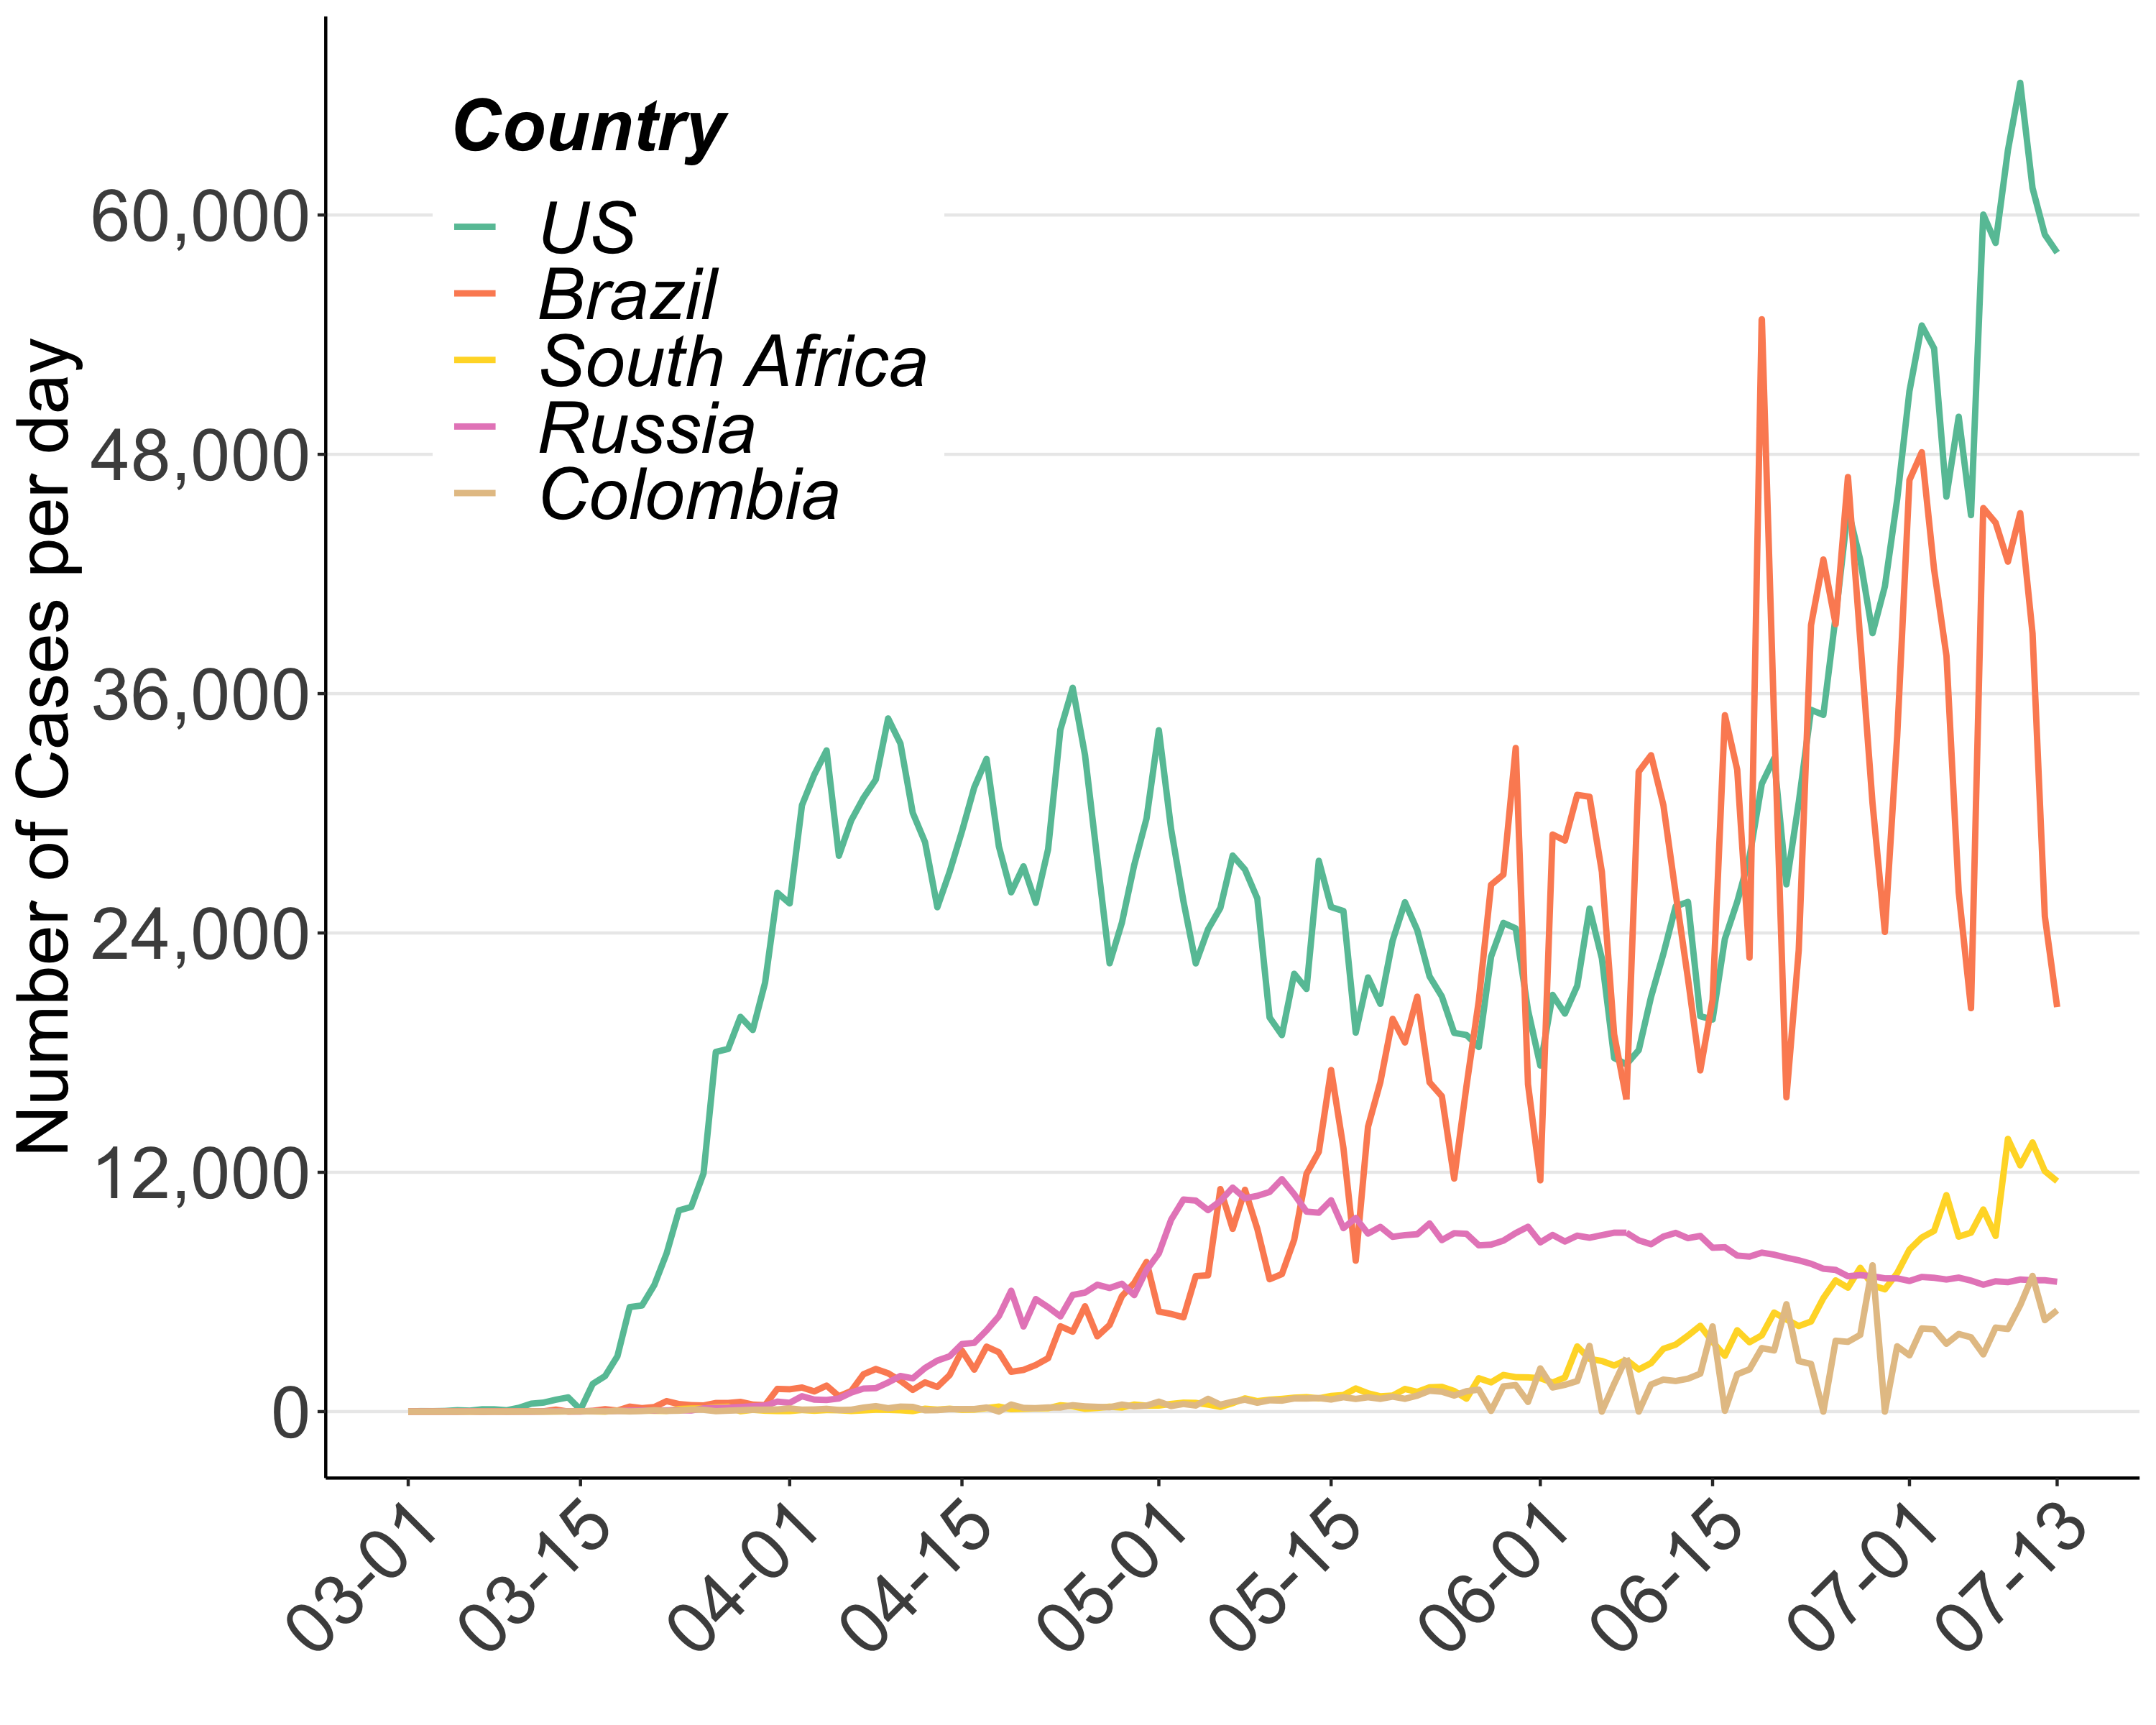
\includegraphics[]{./input/covid2.png}
\label{}
\end{minipage}
\quad
\begin{minipage}[b]{0.45\linewidth}
\caption{日新增死亡病例国家趋势图\\(中国及其他前五位国家) }
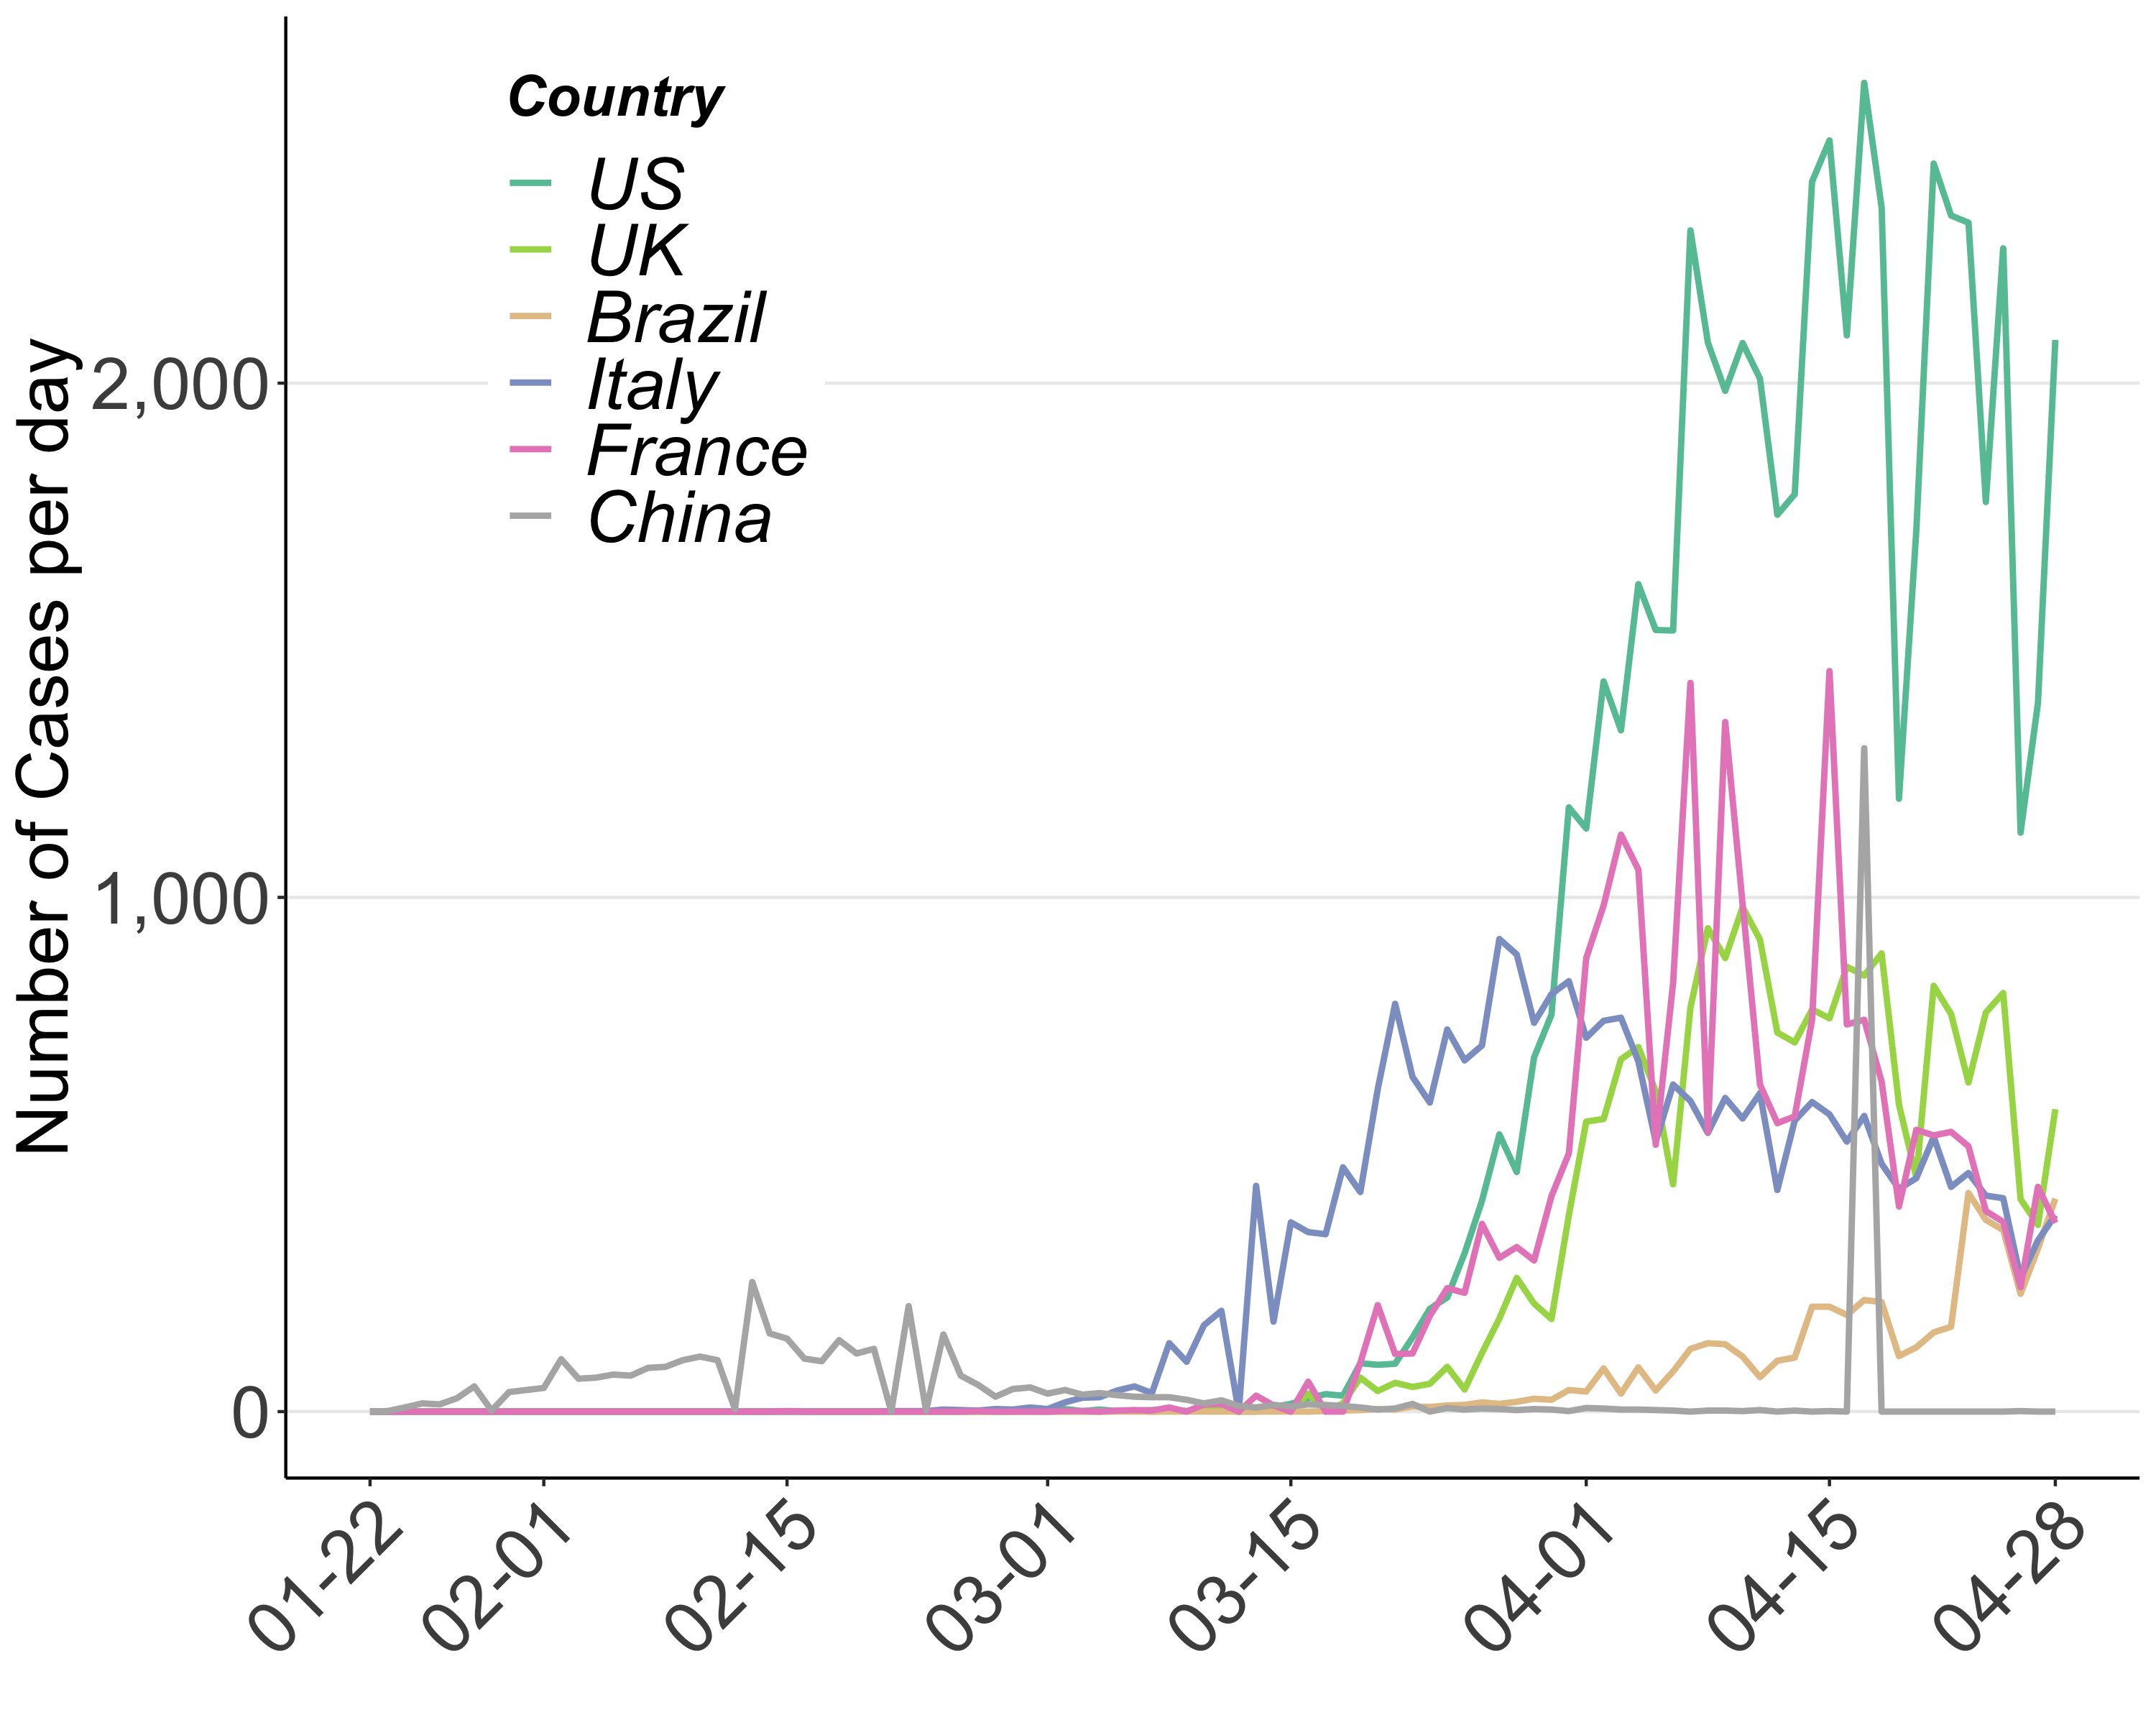
\includegraphics[]{./input/covid3.png}
\label{}
\end{minipage}
\end{figure}

\newpage

\hypertarget{section-3}{%
\section{\texorpdfstring{\textcolor{glaucous}{二、美国疫情}}{}}\label{section-3}}

\vspace{-5mm}

\(\quad\)截至北京时间4月29日早7:00,
美国累计确诊病例数超过101万例(1,011,600),共58,343
死亡病例。从分布来看,疫情主要集中在东西海岸和五大湖地区,全美19个州累计病例数超过一万人。除中部地区以外,东海岸地区疫情也在迅速扩散。罗得岛州累计确诊接近8000例,而粗发病率为全美第四(748/10万人)。(图4)

\(\quad\)纽约州、新泽西州和马萨诸塞州为美国疫情最严重的三个州。纽约州检测率超过4300/10万人,而阳性率下降至35\%,提示疫情逐步得到控制。此外,特拉华州,科罗拉多州与华盛顿特区阳性率均为22\%左右,超过伊利诺伊州,而检测在2000/10万人左右,略低于新泽西州,显示这些州对于检测的需求仍然十分庞大。(表4)

\begin{figure}[H]
\centering
\begin{minipage}[b]{0.45\linewidth}
\caption{美国日新增确诊前五位州趋势图}
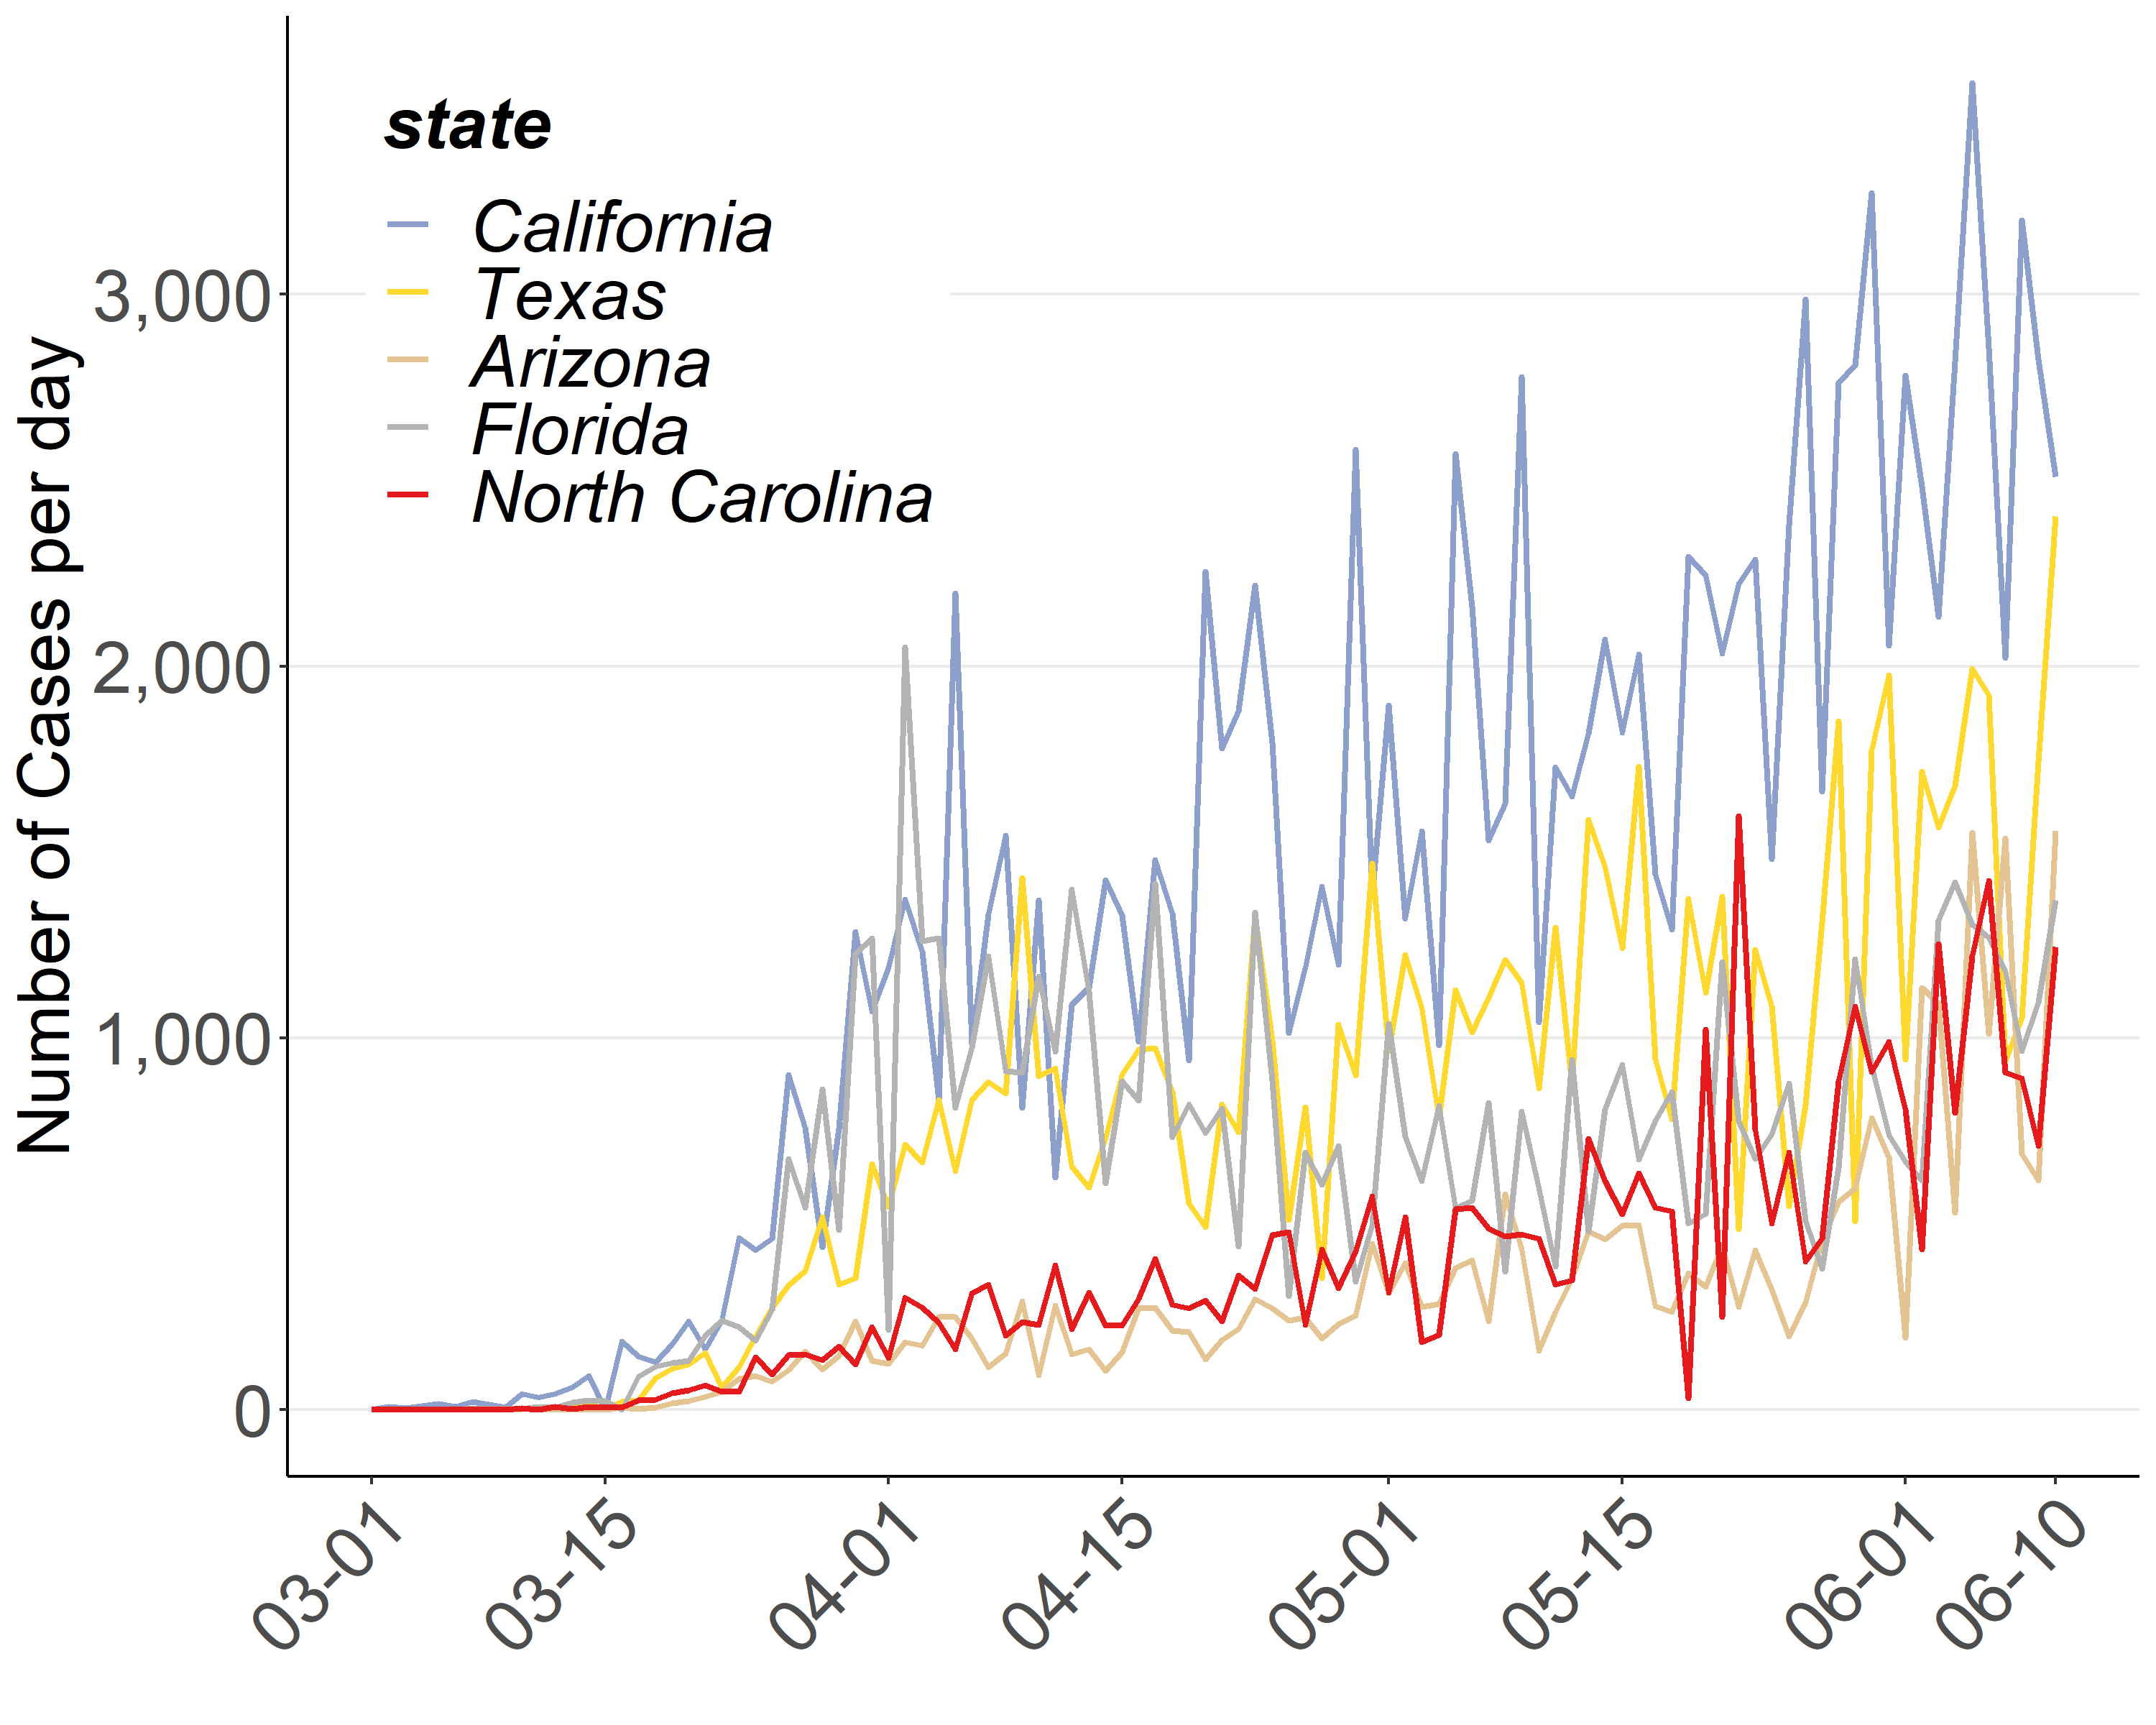
\includegraphics[]{./input/covid5.png}
\label{}
\end{minipage}
\quad
\begin{minipage}[b]{0.45\linewidth}
\caption{美国日新增死亡前五位州趋势图}
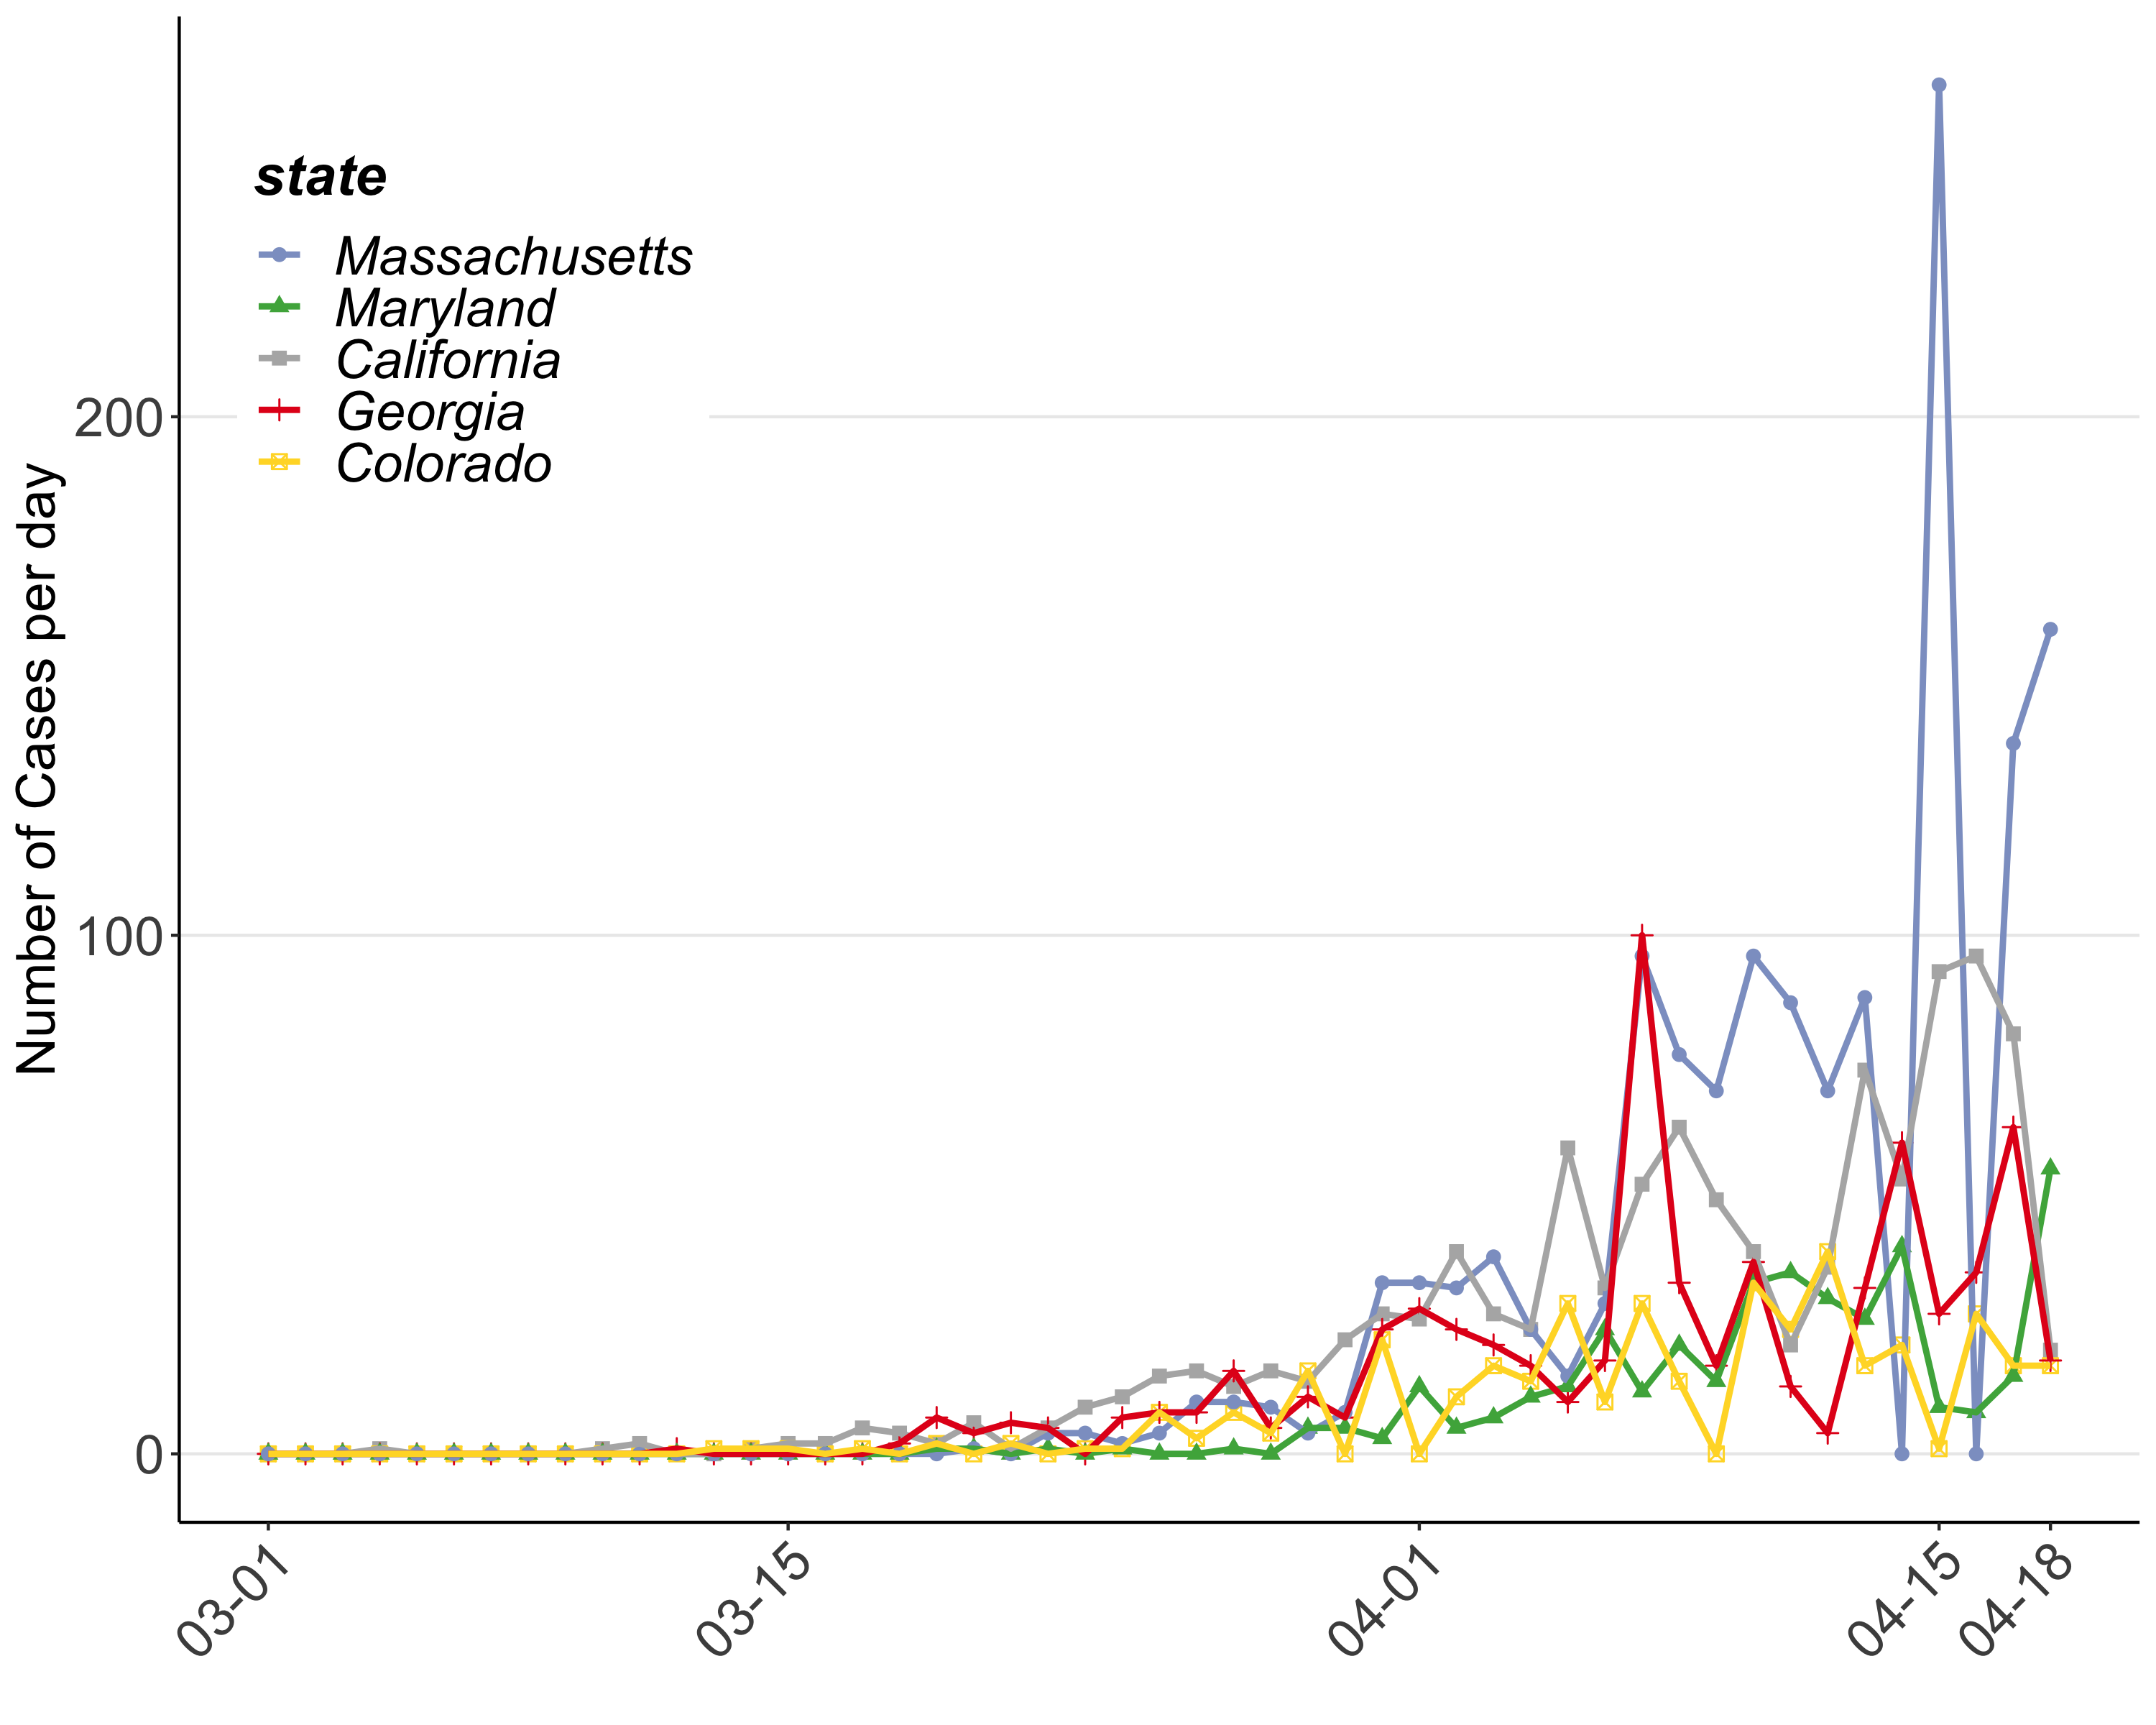
\includegraphics[]{./input/covid6.png}
\label{}
\end{minipage}
\end{figure}

\begin{table}[H]
    \vspace{-7mm}
    \begin{minipage}{.4\linewidth}
    \caption{美国新增确诊前十位州}
    \vspace{0.5\baselineskip}
      \centering
    \captionsetup{justification=centering} \begin{table}[H]
\centering
\begin{tabular}{rlrr}
\toprule
  & 国家/州名 & 当日新增 & 累计确诊\\
\midrule
\rowcolor{gray!6}   & 美国 US & 11,474 & 2,291,353\\
1 & 佛罗里达州 FL & 2,926 & 100,217\\
\rowcolor{gray!6}  2 & 北卡罗莱纳州 NC & 2,224 & 53,614\\
3 & 亚利桑那州 AZ & 2,008 & 54,599\\
\rowcolor{gray!6}  4 & 纽约州 NY & 552 & 388,488\\
5 & 弗吉尼亚州 VA & 471 & 58,465\\
\rowcolor{gray!6}  6 & 路易斯安那州 LA & 461 & 50,239\\
7 & 阿拉巴马州 AL & 433 & 30,454\\
\rowcolor{gray!6}  8 & 宾夕法尼亚州 PA & 366 & 86,301\\
9 & 明尼苏达州 MN & 307 & 33,227\\
\rowcolor{gray!6}  10 & 马里兰州 MD & 297 & 64,603\\
\bottomrule
\end{tabular}
\end{table} \end{minipage}%
    \begin{minipage}{.7\linewidth}
     \caption{美国新增死亡前十位州}
     \vspace{0.5\baselineskip}
      \centering
    \captionsetup{justification=centering} \begin{table}[H]
\centering
\begin{tabular}{rlrrr}
\toprule
  & 国家/州名 & 当日新增 & 累计死亡 & 病死率\%\\
\midrule
\rowcolor{gray!6}   & 美国 US & 137 & 120,106 & 5.2\\
1 & 纽约州 NY & 43 & 31,168 & 8.0\\
\rowcolor{gray!6}  2 & 印第安纳州 IN & 13 & 2,553 & 6.0\\
3 & 佛罗里达州 FL & 12 & 3,173 & 3.2\\
\rowcolor{gray!6}  4 & 路易斯安那州 LA & 12 & 3,117 & 6.2\\
5 & 北卡罗莱纳州 NC & 9 & 1,224 & 2.3\\
\rowcolor{gray!6}  6 & 罗得岛 RI & 9 & 903 & 5.5\\
7 & 弗吉尼亚州 VA & 9 & 1,620 & 2.8\\
\rowcolor{gray!6}  8 & 马里兰州 MD & 8 & 3,074 & 4.8\\
9 & 明尼苏达州 MN & 4 & 1,416 & 4.3\\
\rowcolor{gray!6}  10 & 加利福尼亚州 CA & 3 & 5,518 & 3.1\\
\bottomrule
\end{tabular}
\end{table} \end{minipage} 
\end{table}

\(\quad\)从日新增确诊来看,纽约州单日新增连续多日下降,较昨日再次下降800例左右,提示疫情好转。伊利诺伊州日新增病例逐步上升,需要进一步关注。(表5和图5)

\(\quad\)从死亡病例数来看,密歇根州病死率超过9\%,为全美最高。纽约州与马萨诸塞州日新增死亡呈明显波动下降趋势,提示医疗资源压力得到缓解。值得注意的是,罗得岛州病死率为3\%,略低于佛罗里达州,但其累计病例只有佛罗里达州的1/4(佛罗里达州:32,848例),提示该州存在医疗资源紧张的风险。(表6和图6)

\vspace{5mm}

\centering
\small
\begin{tabular}{ll}

主编:马晶  &  副主编:仁晖\,  薛成海  \\
责任编辑:史珂玮 \, 王冠  \\
新闻组:张宁\, 张心其  & 数据分析:杜兆慧 \\
\multicolumn{2}{l}{可视化组:张立达\, 孙昊\, 唐星鸿\, 齐维为\, 刘逸洋\, 张祺珉\, 周梓淇}

\end{tabular}

\end{document}
